
\begin{frame}
  \frametitle{Models of non-linear regulation}
  \begin{itemize}
  \item <1->Non-linear Activation: Michaelis-Menten Kinetics \[
    \frac{\text{d}x_{i}\left(t\right)}{\text{d}t}=B_{i}+\frac{S_{i}f\left(t\right)}{\gamma_{i}+f\left(t\right)}-D_{i}x_{i}\left(t\right)\]
    used by \citet{Rogers:model06a}
  \item <2->Non-linear Repression \[
    \frac{\text{d}x_{i}\left(t\right)}{\text{d}t}=B_{i}+\frac{S_{i}}{\gamma_{i}+f\left(t\right)}-D_{i}x_{i}\left(t\right)\]
    used by \citealp{Khanin:repression06}, PNAS 103 
  \end{itemize}



\end{frame}

\begin{frame}
  \frametitle{MAP Laplace Approximation}

  Consider the following modification to the model, \[
  \frac{\text{d}x_{j}\left(t\right)}{\text{d}t}=B_{j}+S_{j}g\left(f\left(t\right)\right)-D_{j}x_{j}\left(t\right),\]
  where $g\left(\cdot\right)$ is a non-linear function. The differential
  equation can still be solved, \[
  x_{j}\left(t\right)=\frac{B_{j}}{D_{j}}+S_{j}\int_{0}^{t}e^{-D_{j}\left(t-u\right)}g_{j}\left(f\left(u\right)\right)\text{d}u\]


  Use Laplace's method \citep{Laplace:memoire74}, 
  \[
  p\left(\mathbf{f}\mid\mathbf{x}\right)=N\left(\hat{\mathbf{f}},\mathbf{A}^{-1}\right)\propto\exp\left(-\frac{1}{2}\left(\mathbf{f}-\hat{\mathbf{f}}\right)^{\mbox{T}}\mathbf{A}\left(\mathbf{f}-\hat{\mathbf{f}}\right)\right)
  \]
  where $\hat{\mathbf{f}}=\textrm{argmax}p(\mathbf{f}\mid\mathbf{x})$
  and $\mathbf{A}=-\nabla\nabla\log p\left(\mathbf{f}\mid\mathbf{y}\right)\mid_{\mathbf{f}=\hat{\mathbf{f}}}$
  is the Hessian of the negative posterior at that point. 



\end{frame}

\subsection{Michaelis-Menten Kinetics}

\begin{frame}
  \frametitle{p53 and Michaelis-Menten Kinetics}

  \begin{flushright}
    \textbf{Pei Gao}
    \par\end{flushright}
  \begin{itemize}
  \item The Michaelis-Menten activation model uses the following non-linearity
    \[
    g_{j}\left(f\left(t\right)\right)=\frac{e^{f\left(t\right)}}{\gamma_{j}+e^{f\left(t\right)}},\]
    where we are using a GP $f\left(t\right)$ to model the log of the
    TF activity. %
    \begin{figure}
      \centering{} \label{fig:mlpact:a} 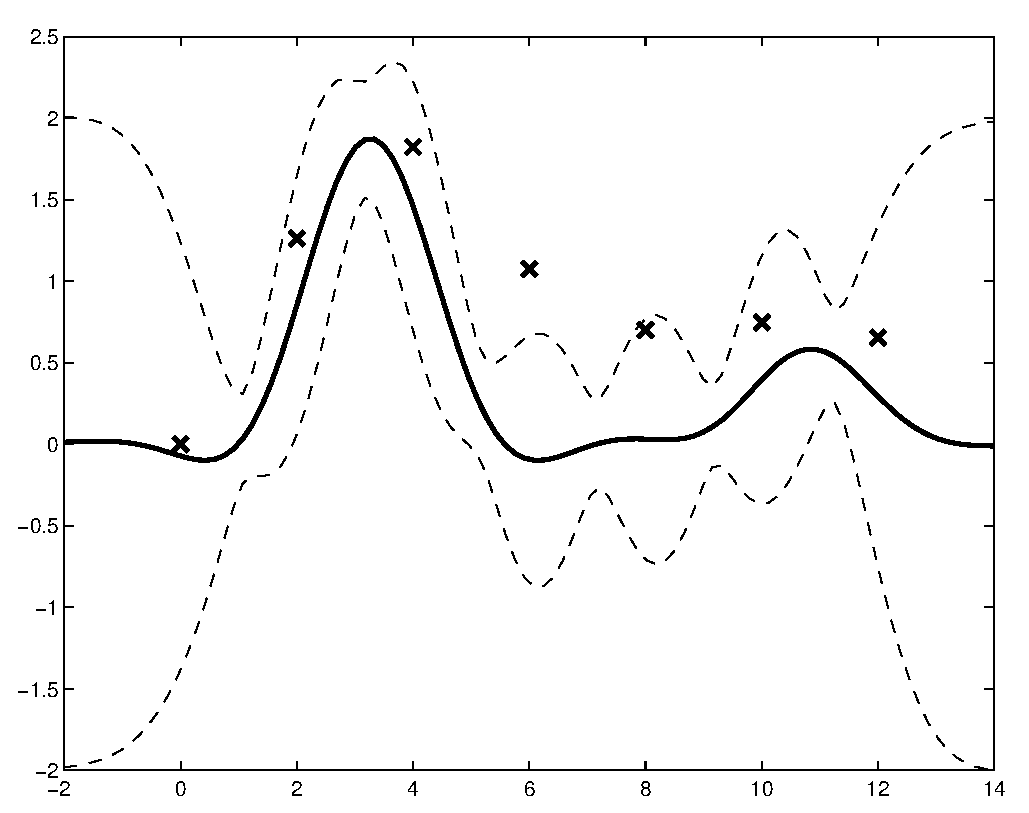
\includegraphics[width=0.35\textwidth]{../../../gpsim/tex/diagrams/demBarenco1_profile3}
      \hfill{}\label{fig:mlpact:b} \subfigure[]{

        \includegraphics[width=0.35\textwidth]{../../../gpsim/tex/diagrams/demBarencoMapMLPAct3_profile3}} 
    \end{figure}

  \end{itemize}

\end{frame}

\begin{frame}
  \frametitle{Valdiation of Laplace Approximation}

  \begin{flushright}
    \textbf{Michalis Titsias}
    \par\end{flushright}

  % 
  \begin{figure}
    \begin{centering}
      \includegraphics[width=0.6\textwidth]{/home/neil/mlprojects/sysbio/tex/diagrams/demBarencoMap1_proteinProfile_Rep3}
      \par\end{centering}

    \caption{Laplace approximation error bars along with samples from the true
      posterior distribution.}

  \end{figure}




\end{frame}

\subsection{MCMC for Non Linear Response}


\begin{frame}
  \frametitle{Use Samples to Represent Posterior}

  \begin{flushright}
    \textbf{Michalis Titsias}
    \par\end{flushright}
  \begin{itemize}
  \item Sample in Gaussian processes\[
    p\left(\mathbf{f}|\mathbf{x}\right)\propto p\left(\mathbf{x}|\mathbf{f}\right)p\left(\mathbf{f}\right)\]

  \item Likelihood relates GP to data through\[
    x_{j}\left(t\right)=\alpha_{j}e^{-D_{j}t}+\frac{B_{j}}{D_{j}}+S_{j}\int_{0}^{t}e^{-D_{j}\left(t-u\right)}g_{j}(f\left(u\right))\text{d}u\]

  \item We use \emph{control points }for fast sampling. {\small \citep{Titsias:efficient08}}
  \end{itemize}

\end{frame}

\begin{frame}
  \frametitle{Sampling using control points}
  \begin{itemize}
  \item Separate the points in $\bff$ into two groups:

    \begin{itemize}
    \item few control points $\bff_{c}$ 
    \item and the large majority of the remaining points $\bff_{\rho}=\bff\setminus\bff_{c}$
    \end{itemize}
  \item Sample the control points $\bff_{c}$ using a proposal $q\left(\bff_{c}^{(t+1)}|\bff_{c}^{(t)}\right)$
  \item Sample the remaining points $\bff_{\rho}$ using the conditional GP
    prior $p\left(\bff_{\rho}^{(t+1)}|\bff_{c}^{(t+1)}\right)$
  \item The whole proposal is \[
    Q\left(\bff^{(t+1)}|\bff^{(t)}\right)=p\left(\bff_{\rho}^{(t+1)}|\bff_{c}^{(t+1)}\right)q\left(\bff_{c}^{(t+1)}|\bff_{c}^{(t)}\right)\]

  \item Its like sampling from the prior $p(\bff)$ but imposing random walk
    behaviour through the control points. 
  \end{itemize}
  \begin{center}

    \par\end{center}


\end{frame}

\begin{frame}
  \frametitle{p53 System Again }
  \begin{itemize}
  \item One transcription factor (p53) that acts as an activator. We consider
    the Michaelis-Menten kinetic equation \[
    \frac{\text{d}x_{j}(t)}{dt}=B_{j}+S_{j}\frac{\exp(f(t))}{\exp(f(t))+\gamma_{j}}-D_{j}x_{j}(t)\]

  \item MCMC details: 

    \begin{itemize}
    \item 7 control points are used (placed in a equally spaced grid) 
    \item Running time 4/5 hours for 2 million sampling iterations plus burn
      in 
    \item Acceptance rate for $\bff$ after burn in was between $15\%-25\%$ 
    \end{itemize}
  \end{itemize}

\end{frame}

\begin{frame}
  \frametitle{Data used by \citet{Barenco:ranked06}: Predicted gene expressions
    for the 1st replica}

  % 
  \begin{figure}
    \centering{}\begin{tabular}{ccc}
      \includegraphics[width=35mm,height=33mm]{../../../gpsim/tex/diagrams/mcmc/demBarencoNoMCMC7RbfexpMichMentenAct_ExprsProfile_Rep1_Gene1} & \includegraphics[width=35mm,height=33mm]{../../../gpsim/tex/diagrams/mcmc/demBarencoNoMCMC7RbfexpMichMentenAct_ExprsProfile_Rep1_Gene2} & \includegraphics[width=35mm,height=33mm]{../../../gpsim/tex/diagrams/mcmc/demBarencoNoMCMC7RbfexpMichMentenAct_ExprsProfile_Rep1_Gene3} \tabularnewline
      \includegraphics[width=35mm,height=33mm]{../../../gpsim/tex/diagrams/mcmc/demBarencoNoMCMC7RbfexpMichMentenAct_ExprsProfile_Rep1_Gene4} & \includegraphics[width=35mm,height=33mm]{../../../gpsim/tex/diagrams/mcmc/demBarencoNoMCMC7RbfexpMichMentenAct_ExprsProfile_Rep1_Gene5}  & \tabularnewline
    \end{tabular}
  \end{figure}



\end{frame}

\begin{frame}
  \frametitle{Data used by \citet{Barenco:ranked06}: Protein concentrations}

  % 
  \begin{figure}
    \centering{}\begin{tabular}{ccc}
      \includegraphics[width=35mm,height=26mm]{../../../gpsim/tex/diagrams/mcmc/demBarencoMCMC2Rbflinear_profile1_slide} & \includegraphics[width=35mm,height=26mm]{../../../gpsim/tex/diagrams/mcmc/demBarencoMCMC2Rbflinear_profile2_slide} & \includegraphics[width=35mm,height=26mm]{../../../gpsim/tex/diagrams/mcmc/demBarencoMCMC2Rbflinear_profile3_slide} \tabularnewline
    \end{tabular}
  \end{figure}


  \begin{center}
    Linear model (Barenco et al. predictions are shown as crosses) %
    \begin{figure}
      \centering{}\begin{tabular}{ccc}
        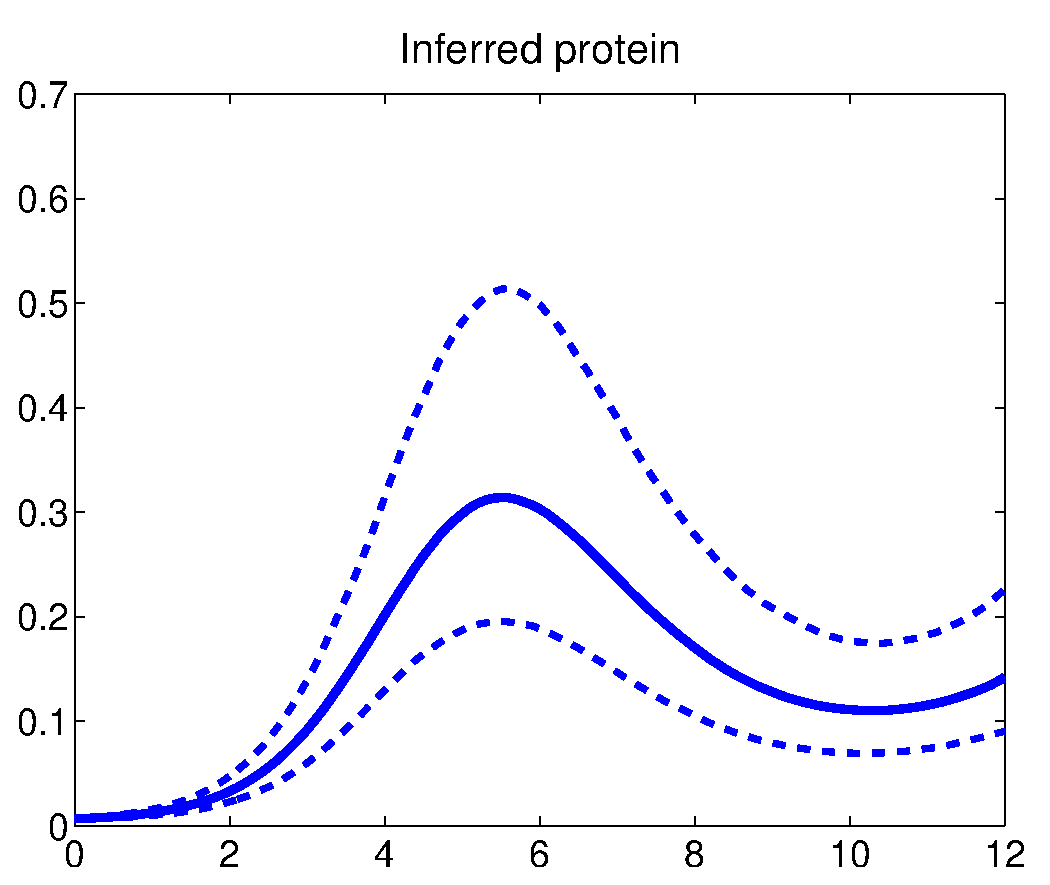
\includegraphics[width=35mm,height=26mm]{../../../gpsim/tex/diagrams/mcmc/demBarencoNoMCMC7RbfexpMichMentenAct_profile1_slide} & \includegraphics[width=35mm,height=26mm]{../../../gpsim/tex/diagrams/mcmc/demBarencoNoMCMC7RbfexpMichMentenAct_profile2_slide} & \includegraphics[width=35mm,height=26mm]{../../../gpsim/tex/diagrams/mcmc/demBarencoNoMCMC7RbfexpMichMentenAct_profile3_slide} \tabularnewline
      \end{tabular}
    \end{figure}

    \par\end{center}

  \begin{center}
    Nonlinear (Michaelis-Menten kinetic equation)
    \par\end{center}


\end{frame}

\begin{frame}
  \frametitle{p53 Data Kinetic parameters}

  % 
  \begin{figure}
    \centering{}\begin{tabular}{cc}
      \includegraphics[width=45mm,height=31mm]{../../../gpsim/tex/diagrams/mcmc/demBarencoWithErrBarsNoMCMC7RbfexpMichMentenAct_basal} & \includegraphics[width=45mm,height=31mm]{../../../gpsim/tex/diagrams/mcmc/demBarencoWithErrBarsNoMCMC7RbfexpMichMentenAct_decay} \tabularnewline
      \includegraphics[width=45mm,height=31mm]{../../../gpsim/tex/diagrams/mcmc/demBarencoWithErrBarsNoMCMC7RbfexpMichMentenAct_sensitivity} & \includegraphics[width=45mm,height=31mm]{../../../gpsim/tex/diagrams/mcmc/demBarencoWithErrBarsNoMCMC7RbfexpMichMentenAct_gamma} \tabularnewline
    \end{tabular}
  \end{figure}


  Our results (grey) compared with \citet{Barenco:ranked06} (black).
  Note that \citeauthor{Barenco:ranked06} use a linear model



\end{frame}

